\documentclass{beamer} 
\usetheme{Boadilla}
\usepackage[brazil]{babel}
\usepackage[active]{srcltx}
\usepackage{latexsym,amsmath,amssymb,amsfonts,amsthm,bm}
\usepackage{natbib}
\usepackage [utf8] {inputenc}
\usepackage[algoruled,noend]{algorithm2e}
\usepackage{graphicx}
\setbeamertemplate{bibliography item}{\insertbiblabel}

\title{Desafio do Bootcamp de Otimização ENACOM 2022}
\author[Fabricio Schiavon Kolberg]{Fabricio Schiavon Kolberg}
\date{Agosto 2022}
\begin{document}

\begin{frame}
\titlepage
\end{frame}

\begin{frame}{Apresentação Pessoal}\pause
Educação:
\begin{itemize}
\item Bacharel em Ciência da Computação na Universidade Federal do Paraná (2008-2013).\pause
\item Mestrado em Informática na Universidade Federal do Paraná (2014-2016).\pause
\item Doutor em Ciência da Computação na Universidade Federal do Paraná (2016-2021).\pause
\end{itemize}
Experiência acadêmica:
\begin{itemize}
\item Teoria da computação.\pause
\item Teoria dos grafos.\pause
\item Métodos formais.\pause
\end{itemize}
Experiência profissional:
\begin{itemize}
\item Estágio: LABMET-UFPR (number crunching com Fortran, análise de dados atmosféricos) (2013-2014).
\end{itemize}
\end{frame}

\begin{frame}{Introdução ao Problema}\pause
Lista de potenciais investimentos:\\
\scriptsize
\pause
\begin{center}
\begin{tabular}{ |cccc| } 
\hline
Opção & Descrição & Custo (R\$) & Retorno (R\$) \\
\hline
\hline
1 & Ampliação da capacidade do armazém ZDP em 5\% & 470.000 & 410.000 \\
2 & Ampliação da capacidade do armazém MGL em 7\% & 400.000 & 330.000 \\
3 & Compra de empilhadeira & 170.000 & 140.000 \\
4 & Projeto de P\&D I & 270.000 & 250.000 \\
5 & Projeto de P\&D II & 340.000 & 320.000 \\
6 & Aquisição de novos equipamentos & 230.000 & 320.000 \\
7 & Capacitação de funcionários & 50.000 & 90.000 \\
8 & Ampliação da estrutura de carga rodoviária & 440.000 & 190.000 \\
\hline
\end{tabular}\pause
\end{center}

\normalsize
Orçamento de R\$ 1.000.000.\pause

Restrições adicionais:\pause
\begin{itemize}
\item Se a opção 1 for selecionada, a opção 5 \textit{não} pode ser.\pause
\item Se a opção 2 for selecionada, a opção 4 \textit{também} deve ser.\pause
\end{itemize}

Desafio: maximizar o retorno de investimento sem quebrar o orçamento máximo, e respeitando as restrições adicionais.

\end{frame}

\begin{frame}{Solução do Problema}
\begin{itemize}
\item Ideia: resolver o problema usando um programa em \emph{Python}.\pause
\item A empresa hipotética pode querer a solução de um problema similar com parâmetros diferentes no futuro.\pause
\item Vale a pena, então, \emph{generalizar} o problema.
\end{itemize}
\end{frame}

\begin{frame}{Versão Generalizada do Problema}
Temos os seguintes dados: \pause
\begin{itemize}
\item $n$ potenciais investimentos $I_1,I_2,...,I_n$.\pause
\item Custos $c_1,c_2,...,c_n$.\pause
\item Retornos $r_1,r_2,...,r_n$.\pause
\item Orçamento máximo disponível $M$.\pause
\end{itemize}
Sejam $v_1,v_2,...,v_n$ as \emph{variáveis de decisão} do problema, onde,
para todo $ 1 \le i \le n$, $v_i = 1$ se o investimento $I_i$ for escolhido, e
$v_i = 0$ caso contrário.\pause

Restrições adicionais:\pause
\begin{description}
\item[Restrições de conflito] Se os investimentos $I_a$ e $I_b$ conflitam, $v_a$ e $v_b$ não podem ambos ser $1$.\pause
\item[Restrições de dependência] Se o investimento $I_a$ depende de $I_b$, então $v_a$ só pode ser $1$ se $v_b$ também for.\pause
\end{description}

\end{frame}

\begin{frame}{Modelagem Matemática}
Função objetivo:
\begin{center}
$\max \sum\limits_{i=1}^n v_ir_i$
\end{center}\pause
Restrição orçamentária:
\begin{center}
$\sum\limits_{i=1}^n v_ic_i \le M$
\end{center}\pause
Restrições de conflito, para todo $1 \le a,b \le n$ tal que $I_a,I_b$ conflitam:
\begin{center}
$v_a+v_b \le 1$
\end{center}\pause
Restrições de dependência, para todo $1 \le a,b \le n$ tal que $I_a$ depende de $I_b$:
\begin{center}
$v_b+(1-v_a) \ge 1$
\end{center}
Domínio das variáveis de decisão:
\begin{center}
$\forall 1 \le i \le n, v_i \in \{0,1\}$.
\end{center}
\end{frame}

\begin{frame}{Modelagem Matemática}
Para o problema do desafio:\pause
\begin{itemize}
\item $n = 8$\pause
\item \footnotesize $c_1 = 470000, c_2 = 400000, c_3 = 170000, c_4 = 270000, c_5 = 340000, c_6 = 230000, c_7=50000,c_8=440000$\pause
\item $r_1 = 410000, r_2 = 330000, r_3 = 140000, r_4 = 250000, r_5 = 320000, r_6 = 320000, r_7=90000,r_8=190000$\normalsize\pause
\item $M = 1000000$\pause
\item $v_1 + v_5 \le 1$\pause
\item $v_4+(1-v_2) \ge 1$
\end{itemize}
\end{frame}

\begin{frame}{Criação do Programa}
\begin{itemize}
\item Utilizando o pacote \emph{science-optimization} do Python.\pause
\item Representação de problemas de otimização do pacote:\\\pause
 $\min f(x)$\\
 Sujeito a:\\
 $g(x) \le 0$\\
 $h(x) = 0$
\end{itemize}
\end{frame}

\begin{frame}{Criação do Programa}
Adaptando as expressões do problema para o \emph{science-optimization}.\pause

Função objetivo:
\begin{center}
$\min \sum\limits_{i=1}^n v_i(-r_i)$
\end{center}\pause

Restrição de orçamento:
\begin{center}
$\sum\limits_{i=1}^n v_ic_i \le M \Rightarrow \sum\limits_{i=1}^n v_ic_i - M \le 0$.
\end{center}\pause

Conflitos:
\begin{center}
$v_a+v_b \le 1 \Rightarrow v_a+v_b - 1 \le 0$
\end{center}\pause

Dependências:
\begin{center}
$v_b+(1-v_a) \ge 1 \Rightarrow -v_b-1+v_a \le -1 \Rightarrow -v_b-1+v_a +1 \le 0 \Rightarrow -v_b+v_a \le 0$
\end{center}
\end{frame}

\begin{frame}{Criação do Programa}
Estruturas de dados básicas para \emph{entrada}:\pause
\begin{description}
\item[Custos] Lista de valores numéricos $[c_1,...,c_n]$.\pause
\item[Retornos] Lista de valores numéricos $[r_1,...,r_n]$.\pause
\item[Orçamento] Valor numérico.\pause
\item[Conflitos] Lista de pares de índices (onde índice $i$ representa o investimento $i+1$) $[[a_1,b_1],...,[a_k,b_k]]$.\pause
\item[Dependências] Lista de pares de índices (onde índice $i$ representa o investimento $i+1$) $[[a_1,b_1],...,[a_l,b_l]]$.
\end{description}
\end{frame}

\begin{frame}{Criação do Programa}
Código de entrada:\pause
\begin{center}
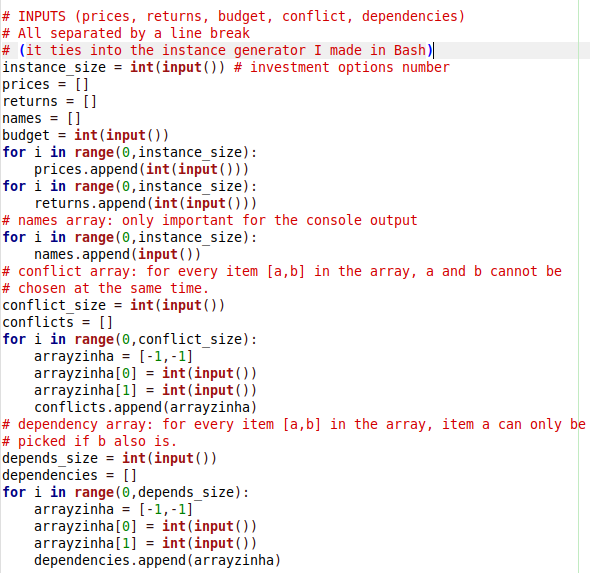
\includegraphics[scale=0.4]{INPUT_CODE_FOR_PRESENTATION.png}
\end{center}
\end{frame}

\begin{frame}{Criação do Programa}
Código de criação do objeto do problema:\pause
\begin{center}
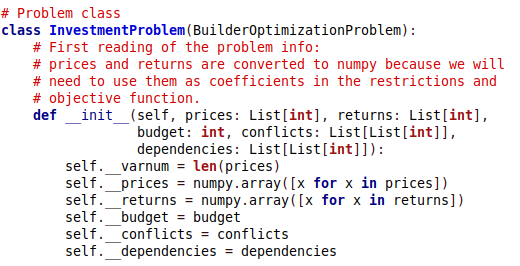
\includegraphics[scale=0.4]{OBJECT_CREATION_FOR_PRESENTATION.png}
\end{center}
\end{frame}

\begin{frame}{Criação do Programa}
Criação das variáveis:\pause
\begin{itemize}
\item Temos $n$ (\_\_varnum) variáveis.\pause
\item Mínimo 0, máximo 1.\pause
\item Variáveis \emph{discretas}.\pause
\end{itemize}
\begin{center}
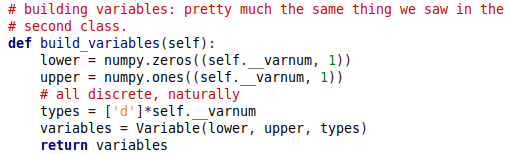
\includegraphics[scale=0.4]{VARIABLES_FOR_PRESENTATION.png}
\end{center}
\end{frame}

\begin{frame}{Criação do Programa}
Expressões de \emph{LinearFunction()} em \emph{science-optimization}:\pause
\begin{center}
$a_1x_1+...+a_nx_n+d$
\end{center}\pause
Sintaxe da função de criação do objeto:\pause
\begin{center}
\emph{LinearFunction($c=[[a_1],...,[a_n]],d=d$)}
\end{center}
\end{frame}

\begin{frame}{Criação do Programa}
Função objetivo: 
\begin{center}
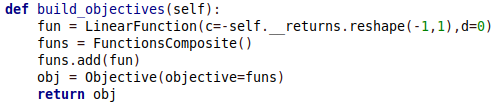
\includegraphics[scale=0.4]{OBJECTIVE_FOR_PRESENTATION.png}
\end{center}\pause
Restrição de orçamento:
\begin{center}
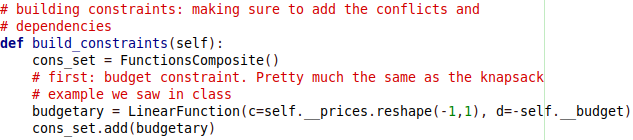
\includegraphics[scale=0.4]{BUDGET_FOR_PRESENTATION.png}
\end{center}
\end{frame}

\begin{frame}{Criação do Programa}
Restrições de conflito e dependência:
\begin{center}
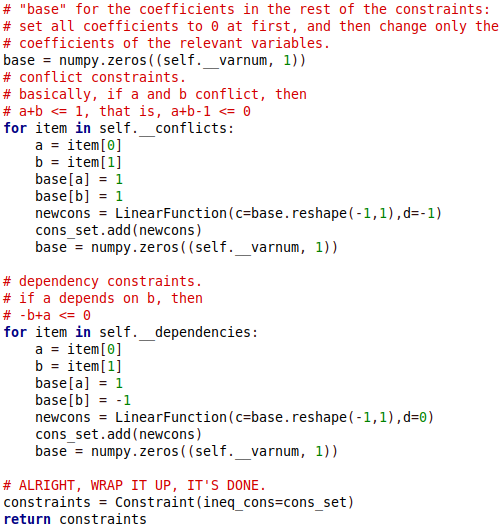
\includegraphics[scale=0.4]{BINARY_RESTRICTIONS_FOR_PRESENTATION.png}
\end{center}
\end{frame}

\begin{frame}{Criação do Programa}
Execução do problema e impressão do resultado:
\begin{center}
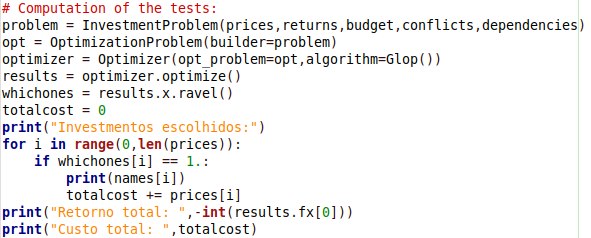
\includegraphics[scale=0.4]{CONCLUSION_FOR_PRESENTATION.png}
\end{center}
\end{frame}

\begin{frame}{Resultados}
Primeiramente, os resultados para o problema do desafio:\pause
\begin{center}
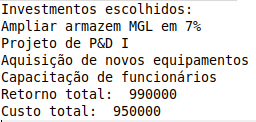
\includegraphics[scale=0.8]{RESULT_FOR_PRESENTATION.png}
\end{center}
\end{frame}

\begin{frame}{Resultados}
Para estudar o desempenho do programa mais a fundo, foi criado um
\emph{gerador de instâncias}.\pause

Para cada número de investimentos entre 1 e 500, dez instâncias foram geradas,
e o tempo de execução médio do programa foi medido para cada uma.
\end{frame}

\end{document}




